\documentclass{ctexbeamer}

\usetheme{Madrid}
\beamertemplatenavigationsymbolsempty

%\usecolortheme{beaver}
% the following colors are modified from beaver
\definecolor{tuna}{rgb}{0.098,0.51,0.996}
\definecolor{thu}{rgb}{0.50,0.36,0.71}

\setbeamercolor{section in toc}{fg=black,bg=white}
\setbeamercolor{item}{fg=tuna,bg=white}
\setbeamercolor{alerted text}{fg=tuna!80!gray}
\setbeamercolor*{palette primary}{fg=tuna!60!black,bg=gray!30!white}
\setbeamercolor*{palette secondary}{fg=tuna!70!black,bg=gray!15!white}
\setbeamercolor*{palette tertiary}{bg=tuna!80!black,fg=gray!10!white}
\setbeamercolor*{palette quaternary}{fg=tuna,bg=gray!5!white}

\setbeamercolor*{sidebar}{fg=tuna,bg=gray!15!white}

\setbeamercolor*{palette sidebar primary}{fg=tuna!10!black}
\setbeamercolor*{palette sidebar secondary}{fg=white}
\setbeamercolor*{palette sidebar tertiary}{fg=tuna!50!black}
\setbeamercolor*{palette sidebar quaternary}{fg=gray!10!white}

%\setbeamercolor*{titlelike}{parent=palette primary}
\setbeamercolor{titlelike}{parent=palette primary,fg=tuna}
\setbeamercolor{frametitle}{bg=gray!10!white}
\setbeamercolor{frametitle right}{bg=gray!60!white}

\setbeamercolor*{separation line}{}
\setbeamercolor*{fine separation line}{}

\setbeamertemplate{sections/subsections in toc}[square]
\setbeamertemplate{items}[square]

% https://tex.stackexchange.com/questions/248131/delete-institute-space-in-title-page-beamer-class
\defbeamertemplate{title page}{noinstitute}[1][]
{
  \vbox{}
  \vfill
  \begingroup
    \centering
    \begin{beamercolorbox}[sep=8pt,center,#1]{title}
      \usebeamerfont{title}\inserttitle\par%
      \ifx\insertsubtitle\@empty%
      \else%
        \vskip0.25em%
        {\usebeamerfont{subtitle}\usebeamercolor[fg]{subtitle}\insertsubtitle\par}%
      \fi%     
    \end{beamercolorbox}%
    \vskip1em\par
    \begin{beamercolorbox}[sep=8pt,center,#1]{author}
      \usebeamerfont{author}\insertauthor
    \end{beamercolorbox}
    \begin{beamercolorbox}[sep=8pt,center,#1]{date}
      \usebeamerfont{date}\insertdate
    \end{beamercolorbox}\vskip0.5em
    {\usebeamercolor[fg]{titlegraphic}\inserttitlegraphic\par}
  \endgroup
  \vfill
}

\makeatletter
\setbeamertemplate{title page}[noinstitute][colsep=-4bp,rounded=true,shadow=\beamer@themerounded@shadow]
\makeatother

\usepackage{tikz}
\usetikzlibrary{arrows}
\usepackage{hyperref}

\setCJKmainfont{Source Han Sans CN}
\setCJKsansfont{Source Han Sans CN}
\setCJKmonofont{Source Han Sans CN}

\newcommand{\T}[1]{\texttt{#1}}

\title[Mirror\{S,Z\}]{MirrorZ:从镜像站到镜像站们}
\author[Zenithal]{Zenithal\newline\url{hongren.zheng@tuna.tsinghua.edu.cn}}
\date{2021-09-25}
\titlegraphic{\includegraphics[width=0.8\textwidth]{img/logo3.png}}

\begin{document}

\begin{frame}
\titlepage
\end{frame}

\begin{frame}{关于我}
  \begin{columns}
    \begin{column}{0.65\textwidth}
      \begin{itemize}
        \item 关于我\begin{itemize}
          \item 头像是綾波レイ
          \item 曾经的头像是初音未来
          \item GitHub:\url{ZenithalHourlyRate}
          \item GPG:\url{blog.zenithal.me/key}
          \item 更多介绍在 GitHub 的 README 中
        \end{itemize}
        \item 在金枪鱼(TUNA)中\begin{itemize}
          \item 潜水摸鱼两三年
          \item 「(2020年)11月,zenithal 开始加入到镜像站的维护中。」(引自 \url{tuna.wiki/MirrorsHistory})
        \end{itemize}
      \end{itemize}
      \begin{figure}
        \centering
        \includegraphics[width=0.8\textwidth]{img/contri.png}
      \end{figure}
    \end{column}
    \begin{column}{0.35\textwidth}
      \includegraphics[width=0.9\textwidth]{img/rei.jpg}
      \includegraphics[width=0.9\textwidth]{img/miku.jpg}
    \end{column}
  \end{columns}
\end{frame}

\section{镜像站}
\begin{frame}{镜像站维护,具体在做啥}
  \begin{itemize}
    \item \url{tuna/issues}:镜像请求,问题反馈\begin{itemize}
      \item 打打杂、关关 issue
    \end{itemize}
    \item \T{tuna/mirror-web}:镜像站前端,帮助文档,合 Pull Request
    \item \T{tuna/tunasync}:同步管理工具
    \item \T{tuna/tunasync-scripts}:同步脚本\begin{itemize}
      \item 例如修理 \T{homebrew-bottles} 同步脚本
    \end{itemize}
    \item \T{tuna/collection}:讲段子
  \end{itemize}
  \begin{figure}
    \centering
    \includegraphics[width=0.9\textwidth]{img/666.png}
  \end{figure}
\end{frame}

\begin{frame}{镜像站维护,好做吗}
  \begin{itemize}
    \item \url{tuna/issues}:镜像请求,问题反馈\begin{itemize}
      \item 打打杂、关关 issue
      \item 其实会参考隔壁镜像站的情况
      \includegraphics[width=0.5\textwidth]{img/ustc-discuss.png}
    \end{itemize}
    \item \T{tuna/mirror-web}:镜像站前端,帮助文档,合 Pull Request\begin{itemize}
      \item 参考隔壁镜像站的帮助文档
    \end{itemize}
    \item \T{tuna/tunasync-scripts}:同步脚本\begin{itemize}
      \item 例如修理 \T{homebrew-bottles} 同步脚本,具体工作内容就是照抄 USTC 的同步脚本
    \end{itemize}
    \item 工作流其实有问题\begin{itemize}
      \item 遇到新问题,会遍历一次隔壁镜像站(USTC/SJTUG等)
      \item 新镜像请求,有时候甚至不知道友镜有没有这个镜子,得遍历主页
    \end{itemize}
  \end{itemize}
\end{frame}

\begin{frame}{镜像站维护带来的启发}
  \begin{columns}
    \begin{column}{0.55\textwidth}
      \begin{itemize}
        \item 镜像站管理员想要找东西,都要遍历各个镜像站,更何况是用户
        \item 如果用户找 rocky 镜像站的时候能有右边的面板,会方便很多
        \item 更进一步,如果在「换源」时自动选择最优镜像,那该多方便
      \end{itemize}
    \end{column}
    \begin{column}{0.45\textwidth}
      \includegraphics[width=0.9\textwidth]{img/rocky.png}
    \end{column}
  \end{columns}
\end{frame}

\section{镜像站们}
\begin{frame}{镜像站们}
  \begin{itemize}
    \item 基于上述情况,我和各镜像站的管理员、用户,开发了 MirrorZ(中文名暂为「镜像站们」)
    \item 如果用户找 rocky 镜像站的时候能有上页的面板,会方便很多\begin{itemize}
      \item 前端:可供用户查询「常用软件」「镜像列表」「镜像站状态」
      %\item 样例在 \url{https://mirrorz.org/}
      %\item 样例在 \url{https://mirrors.cngi.edu.cn/}
    \end{itemize}
    \item 更进一步,如果在「换源」时自动选择最优镜像,那该多方便\begin{itemize}
      \item 跳转后端
      %\item 样例在 \url{https://mirrors.cngi.edu.cn/}
    \end{itemize}
  \end{itemize}
  \begin{figure}
    \centering
    \includegraphics[width=0.45\textwidth]{img/archlinux.png}
    \qquad
    \includegraphics[width=0.45\textwidth]{img/ustc-status.png}
  \end{figure}
\end{frame}

\begin{frame}{MirrorZ 名字的来历}
  \begin{itemize}
    \item 本质原因:没有 mirrors 的域名(例如 mirrors.moe),我只能想一个别的名字
    \item Z 来自我的 ID:Zenithal
    \item Mirrors 的复数形式,与其用 Mirrorses,不如用 Mirrorz\begin{itemize}
      \item Your next MirrorS is not MirrorS, nor MirrorSes, it's MirrorZ.
      \item 你的下一个镜像站何必是镜像站
      \item (跳转后端确实不是镜像站)
    \end{itemize}
    \item 字母表的最后一个字母:A final site for Mirror sites.
    \item 最终决定因素:mirrorz.org 还没有被注册
  \end{itemize}
\end{frame}

\subsection{前端}
\begin{frame}{前端技术细节}
  \begin{itemize}
    \item 各个站的前端、后端各不相同
    \item 同步管理器\begin{itemize}
      \item \T{tuna/tunasync}: \T{tunasync.json}
      \item \T{ustclug/Yuki}: \T{meta}
      \item \T{sjtug/mirror-clone}: \T{summary.json}
      \item \T{ideal/mirror}: \T{task\_status.json}
    \end{itemize}
    \item 首页是 Nginx autoindex:\T{DOMParser} 启动!
    \item 把上述数据转化为统一的 \T{mirrorz.json},即可被前端使用
    \item (该数据格式还被不少 MirrorZ 的下游项目使用,后续会展开)
  \end{itemize}
\end{frame}

\begin{frame}{前端架构}
   联邦式前端 
   \centering
   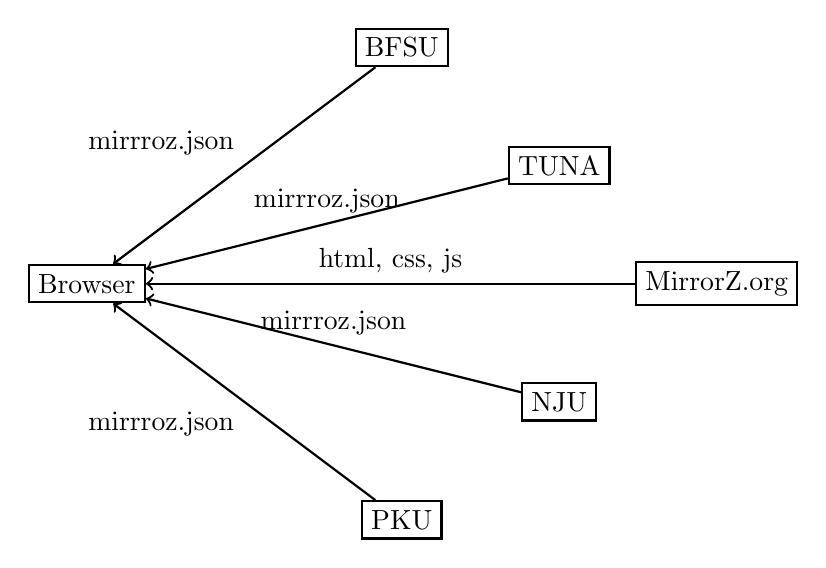
\begin{tikzpicture}[x=2cm, y=1.5cm]
      \node[draw,thick,fill=white] (browser) at (-2, 0) {Browser};
      \node[draw,thick,fill=white] (mirrorz) at (2, 0) {MirrorZ.org};
      \node[draw,thick,fill=white] (TUNA) at (1, 1) {TUNA};
      \node[draw,thick,fill=white] (BFSU) at (0, 2) {BFSU};
      \node[draw,thick,fill=white] (NJU) at (1, -1) {NJU};
      \node[draw,thick,fill=white] (PKU) at (0, -2) {PKU};
      \draw[->,thick] (mirrorz) -- node [above] {html, css, js}  (browser);
      \draw[->,thick] (TUNA) -- node [above] {mirrroz.json}  (browser);
      \draw[->,thick] (BFSU) -- node [above left] {mirrroz.json}  (browser);
      \draw[->,thick] (NJU) -- node [above] {mirrroz.json}  (browser);
      \draw[->,thick] (PKU) -- node [below left] {mirrroz.json}  (browser);
   \end{tikzpicture}
\end{frame}

\begin{frame}{前端部署}
  \begin{center}
    \includegraphics[width=0.7\textwidth]{img/logo3.png}
  \end{center}
  \begin{itemize}
    \item 主站:\url{mirrorz.org}
    \item 教育网分站:\url{mirrors.cngi.edu.cn}\begin{itemize}
      \item 只包含以 edu.cn 结尾的镜像站
    \end{itemize}
    \item 各省份分站 \url{mirrors.xx.cn},例如 \url{mirrors.bj.cn}\begin{itemize}
      \item 如果那个省有镜像站且被 mirrorz 收录
    \end{itemize}
    \item DN42 站: \url{mirror.z.dn42}\begin{itemize}
      \item 虽然里面只有一个镜像站 \url{mirrors.nia.dn42}
    \end{itemize}
  \end{itemize}
\end{frame}

\subsection{跳转后端}
\begin{frame}{跳转后端:如何使用}
  \begin{itemize}
    \item Arch Linux: \T{Server = https://mirrors.cngi.edu.cn/archlinux/\$repo/os/\$arch}
    \item Debian: \T{deb https://mirrors.cngi.edu.cn/debian/ bullseye main contrib non-free}
    \item Ubuntu: \T{deb https://mirrors.cngi.edu.cn/ubuntu/ focal main restricted universe multiverse}
    \item CentOS/Fedora: \T{baseurl=https://mirrors.cngi.edu.cn}
    \item 以及更多软件源,不一而足。「镜像列表」中所列镜像基本可以使用该功能。
  \end{itemize}
\end{frame}

\begin{frame}{跳转后端:打分机制}
  \begin{itemize}
    \item 跳转后端位于镜像站与用户中间,需要考虑两边的因素
    \item 镜像站端\begin{itemize}
      \item 网络环境:接入点,IPv6/IPv4,HTTP/HTTPS,所在网段与AS
      \item 同步状态:各个镜像源的同步情况(同步落后/同步中)
    \end{itemize}
    \item 用户端\begin{itemize}
      \item 网络环境:IPv6/IPv4,HTTP/HTTPS,所在网段与AS
      \item 用户喜好(可选):用户访问时提供喜好列表\begin{itemize}
        \item 用户可以直接使用 mirrors.cngi.edu.cn
        \item 也可使用 ustc-tuna.mirrors.cngi.edu.cn 提供其喜好列表
      \end{itemize}
    \end{itemize}
    \item \T{mirrorz.d.json}: 对 \T{mirrorz.json} 的一个扩展,包含节点的网络环境
    \item 打分机制:对网络环境的匹配情况、用户喜好、同步状态进行打分,占优者会被选择
    \item 可以用 \url{mirrors.cngi.edu.cn/archlinux?trace} 查看技术细节
  \end{itemize}
\end{frame}

\begin{frame}{跳转后端架构}
   \centering
   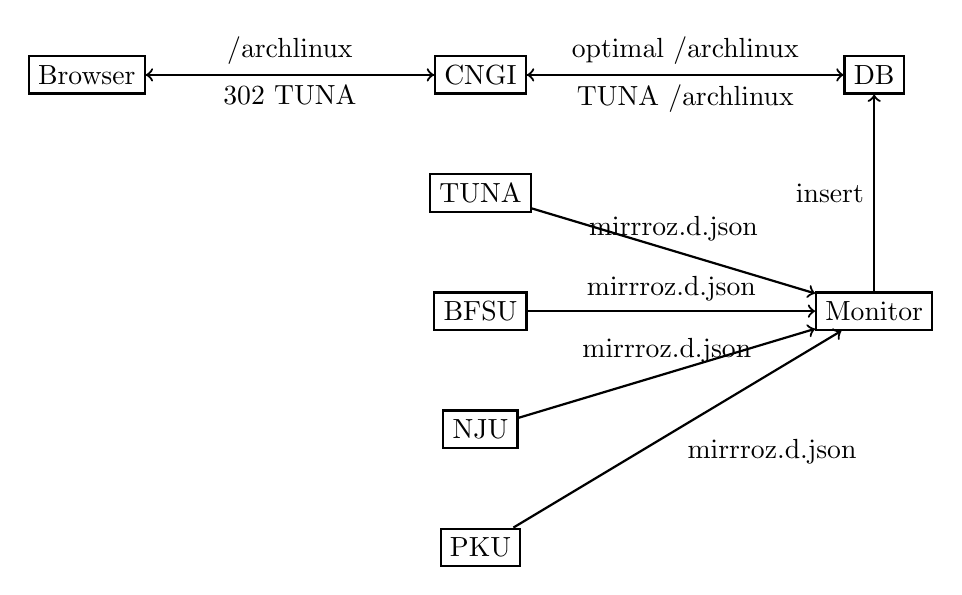
\begin{tikzpicture}[x=2.5cm, y=1.5cm]
      \node[draw,thick,fill=white] (browser) at (-2, 0) {Browser};
      \node[draw,thick,fill=white] (mirrorz) at (0, 0) {CNGI};
      \node[draw,thick,fill=white] (DB) at (2, 0) {DB};
      \node[draw,thick,fill=white] (MON) at (2, -2) {Monitor};
      \node[draw,thick,fill=white] (TUNA) at (0, -1) {TUNA};
      \node[draw,thick,fill=white] (BFSU) at (0, -2) {BFSU};
      \node[draw,thick,fill=white] (NJU) at (0, -3) {NJU};
      \node[draw,thick,fill=white] (PKU) at (0, -4) {PKU};
      \draw[->,thick] (browser) -- node [above] {/archlinux}  (mirrorz);
      \draw[->,thick] (mirrorz) -- node [above] {optimal /archlinux}  (DB);
      \draw[->,thick] (DB) -- node [below] {TUNA /archlinux}  (mirrorz);
      \draw[->,thick] (mirrorz) -- node [below] {302 TUNA}  (browser);
      \draw[->,thick] (MON) -- node [left] {insert}  (DB);
      \draw[->,thick] (TUNA) -- node [above] {mirrroz.d.json}  (MON);
      \draw[->,thick] (BFSU) -- node [above] {mirrroz.d.json}  (MON);
      \draw[->,thick] (NJU) -- node [above] {mirrroz.d.json}  (MON);
      \draw[->,thick] (PKU) -- node [below right] {mirrroz.d.json}  (MON);
   \end{tikzpicture}
\end{frame}

\begin{frame}{跳转后端:一些指标}
  \begin{itemize}
    \item 以上打分机制只适用于单次请求,是用户喜好、网络环境与同步状态等因素的折中与妥协
    \item 对于多次请求,我们提出以下指标
    \item 一致性\begin{itemize}
      \item 对于用户单次 \texttt{apt-get update},其跳转的镜像站要保持一致
      \item 以保证其元数据的一致性,避免跳转到的两个镜像站的状态不一致导致用户本地元数据损坏
      \item 实现方式:只需要对用户短时间内的请求做缓存
    \end{itemize}
    \item 单调性\begin{itemize}
      \item 对于用户连续两次 \texttt{apt-get update}请求,新请求获得的版本不会比旧请求的版本更低
      \item 避免本地软件包降级
      \item 实现方式:较难实现或无法实现
    \end{itemize}
    \item 还有一些性能方面的指标,略过不表
  \end{itemize}
\end{frame}

\begin{frame}{跳转后端:部署}
  教育网分站:\url{mirrors.cngi.edu.cn}\begin{itemize}
    \item 跳转后端服务是教育网分站的特色服务
  \end{itemize}
  \begin{figure}
    \centering
    \includegraphics[width=0.9\textwidth]{img/mrzdjson.png}
  \end{figure}
\end{frame}

\begin{frame}{镜像站们:下游项目}
  \begin{columns}
    \begin{column}{0.6\textwidth}
      \begin{itemize}
        \item 有了 mirrorz.json ,可以玩很多花样
        \item \T{oh-my-mirrorz}: 测速脚本!\begin{itemize}
          \item \url{mirrorz.org/oh-my-mirrorz.py}
          \item \url{mirrors.cngi.edu.cn/oh-my-mirrorz.py}
        \end{itemize}
        \item \T{mirrorz-legacy}:静态页面\begin{itemize}
          \item \url{mirrorz.org/\_/}
          \item \url{mirrors.cngi.edu.cn/\_/}
        \end{itemize}
        \item \T{mirrorz-monitor}:镜像状态监控\begin{itemize}
          \item \url{mirrorz.org/monitor}
          \item \url{mirrors.cngi.edu.cn/monitor}
        \end{itemize}
      \end{itemize}
    \end{column}
    \begin{column}{0.4\textwidth}
      \includegraphics[width=0.9\textwidth]{img/speed.png}
    \end{column}
  \end{columns}
\end{frame}

\begin{frame}{镜像站们:后续计划}
  \begin{itemize}
    \item 更多镜像站的参与!\begin{itemize}
      \item \url{mirrorz.org} 包含的大多是国内高校镜像站
      \item 仅校内的镜像站也可以参与到跳转后端中
    \end{itemize}
    \item 更多的下游项目\begin{itemize}
      \item 例如镜像帮助乃至「自动换源」,我们还没有启动 mirrorz-help 项目
      \item 各个镜像站的镜像帮助其实非常相似,只需要做变量替换
    \end{itemize}
    \item 更多的用户:跳转后端的功能、性能如何,还需要测试与反馈
    \item[]\ 
    \item 项目地址,欢迎点星星和贡献代码!\begin{itemize}
      \item 前端:\url{github.com/mirrorz-org/mirrorz}
      \item 跳转后端:\url{github.com/mirrorz-org/mirrorz-302}
    \end{itemize}
  \end{itemize}
\end{frame}

\end{document}

% vim: nospell
